% ============================================================================
% CrowdROM Pipeline: Algorithms and Mathematical Formulation
% ============================================================================
\documentclass[11pt]{article}

% ---- Packages ----
\usepackage[margin=1in]{geometry}
\usepackage{amsmath, amssymb, amsthm}
\usepackage{algorithm}
\usepackage{algpseudocode}
\usepackage{booktabs}
\usepackage{tikz}
\usetikzlibrary{arrows.meta, positioning, calc, fit, backgrounds, shapes.geometric}
\usepackage{hyperref}
\usepackage{natbib}
\usepackage{xcolor}

% ---- Custom commands ----
\newcommand{\R}{\mathbb{R}}
\newcommand{\bx}{\mathbf{x}}
\newcommand{\ba}{\mathbf{a}}
\newcommand{\by}{\mathbf{y}}
\newcommand{\bU}{\mathbf{U}}
\newcommand{\bA}{\mathbf{A}}
\newcommand{\bI}{\mathbf{I}}
\newcommand{\bmu}{\boldsymbol{\mu}}
\newcommand{\brho}{\boldsymbol{\rho}}
\DeclareMathOperator*{\argmax}{arg\,max}
\DeclareMathOperator*{\argmin}{arg\,min}

\title{%
  \textbf{CrowdROM: Shift-Aligned POD--MVAR Pipeline}\\[6pt]
  \large Algorithms for Density-Field Reduced-Order Modeling\\
  with Hellinger Embedding and Simplex Mass Correction}
\author{Macias-Olivares, E.}
\date{February 2026}

\begin{document}
\maketitle

% ============================================================================
\section{Problem Setting}
% ============================================================================

We consider $N$ interacting agents on a periodic domain
$\Omega = [0, L_x) \times [0, L_y)$ evolving under
a discrete-time Vicsek--Morse model \citep{Vicsek1995,DorsognaEtAl2006}.
At each time $t_k = k\,\Delta t$, the particle positions are
$\{\bx_i^k\}_{i=1}^{N} \subset \Omega$.

We construct a \emph{density representation} by binning and smoothing:
\begin{equation}\label{eq:kde}
  \rho^k(x,y)
  \;=\;
  \bigl(G_\sigma * H^k\bigr)(x,y),
  \qquad
  H^k_{jl}
  = \frac{1}{\Delta x\,\Delta y}
    \sum_{i=1}^{N} \mathbf{1}\bigl[\bx_i^k \in C_{jl}\bigr],
\end{equation}
where $H^k \in \R^{N_y \times N_x}$ is the histogram on cells
$C_{jl} = [x_j, x_{j+1}) \times [y_l, y_{l+1})$
with spacing $\Delta x = L_x / N_x$, $\Delta y = L_y / N_y$,
and $G_\sigma$ is a 2D Gaussian kernel with bandwidth~$\sigma$
(in grid-cell units), applied with \emph{periodic wrapping}
\citep{SilvermanKDE1986}.
The density satisfies $\sum_{jl} \rho^k_{jl}\,\Delta x\,\Delta y = N$.

% ---- Implementation note ----
In code, this is \texttt{density.compute\_density\_grid()} using
\texttt{scipy.ndimage.gaussian\_filter} with \texttt{mode='wrap'}.

We flatten each density frame to a column vector
$\brho^k \in \R^n$, $n = N_x N_y$,
and collect $M$ training trajectories of $T$ subsampled frames each into the
\emph{snapshot matrix}
$\mathbf{X}_{\mathrm{raw}} = [\brho^1_1, \ldots, \brho^T_1,\;\ldots,\;\brho^1_M, \ldots, \brho^T_M]^\top \in \R^{MT \times n}.$


% ============================================================================
\section{Step 1: Shift Alignment (sPOD)}
\label{sec:shift_align}
% ============================================================================

Particle systems with net translational motion produce density fields that
\emph{drift} across $\Omega$.  Standard POD is inefficient for traveling
structures: a simple translation requires many Fourier-type modes to
represent \citep{ReissEtAl2018,BlackVellaReiss2020}.

\textbf{Shifted POD (sPOD)} factors out integer-pixel translations
\emph{before} computing the POD basis, so that the reduced coordinates
only need to capture structural deformation.

\subsection{FFT Cross-Correlation Registration}

Given a reference field $\rho_{\mathrm{ref}} \in \R^{N_y \times N_x}$
and a target frame $\rho^k$, we seek the cyclic shift
$(\delta_y^k, \delta_x^k) \in \mathbb{Z}^2$ that maximises the
cross-correlation:
\begin{equation}\label{eq:xcorr}
  (\delta_y^k, \delta_x^k)
  \;=\;
  \argmax_{(s_y, s_x) \in \mathbb{Z}_{N_y} \times \mathbb{Z}_{N_x}}
  \sum_{j,l} \rho_{\mathrm{ref}}(j, l)\;\rho^k\!\bigl((j+s_y)\!\!\mod N_y,\;(l+s_x)\!\!\mod N_x\bigr).
\end{equation}
By the convolution theorem on the periodic domain, this is computed in
$O(n \log n)$ via the 2D FFT:
\begin{equation}\label{eq:xcorr_fft}
  C = \mathcal{F}^{-1}\!\bigl[\mathcal{F}[\rho_{\mathrm{ref}}]
      \odot \overline{\mathcal{F}[\rho^k]}\bigr],
  \qquad
  (\delta_y^k, \delta_x^k) = \argmax_{(s_y, s_x)} \operatorname{Re}(C_{s_y, s_x}),
\end{equation}
where $\overline{(\cdot)}$ denotes elementwise complex conjugation and
$\odot$ is the Hadamard product.
The shift is converted to signed integers by wrapping indices exceeding
$N_y/2$ or $N_x/2$.

\subsection{Alignment and Un-alignment}

The aligned frame is obtained by cyclic rolling:
\begin{equation}\label{eq:roll}
  \tilde{\rho}^k(j, l) = \rho^k\!\bigl((j - \delta_y^k)\!\!\mod N_y,\;
  (l - \delta_x^k)\!\!\mod N_x\bigr).
\end{equation}
At prediction time, forecasted (aligned) fields are \emph{un-aligned}
by applying the \emph{negative} shift:
\begin{equation}
  \hat{\rho}^k_{\mathrm{phys}}(j,l)
  = \hat{\tilde{\rho}}^k\bigl((j + \delta_y^k)\!\!\mod N_y,\;
    (l + \delta_x^k)\!\!\mod N_x\bigr).
\end{equation}
For forecast frames beyond the teacher-forced window, shifts are
\emph{linearly extrapolated}:
$\hat{\boldsymbol{\delta}}(t) = \mathbf{c}_0 + \mathbf{c}_1\, t$, fit by
least-squares to the known shifts.

\begin{algorithm}[t]
\caption{Shift Alignment (sPOD) — Training}
\label{alg:shift_align_train}
\begin{algorithmic}[1]
\Require Snapshot matrix $\mathbf{X}_{\mathrm{raw}} \in \R^{MT \times n}$
  reshaped as $\{\rho^k\}_{k=1}^{MT}$, each $\rho^k \in \R^{N_y \times N_x}$
\Ensure Aligned snapshots $\{\tilde{\rho}^k\}$, reference $\rho_{\mathrm{ref}}$,
  shift array $\boldsymbol{\Delta} \in \mathbb{Z}^{MT \times 2}$
\Statex
\State $\rho_{\mathrm{ref}} \gets \frac{1}{MT}\sum_{k=1}^{MT} \rho^k$
  \Comment{\texttt{shift\_align\_ref='mean'}}
\For{$k = 1, \ldots, MT$}
  \State $\hat{F}_{\mathrm{ref}} \gets \texttt{fft2}(\rho_{\mathrm{ref}})$;\;
         $\hat{F}_k \gets \texttt{fft2}(\rho^k)$
  \State $C \gets \operatorname{Re}\!\bigl(\texttt{ifft2}(\hat{F}_{\mathrm{ref}} \odot \bar{\hat{F}}_k)\bigr)$
  \State $(\delta_y^k, \delta_x^k) \gets \argmax_{(s_y,s_x)} C_{s_y, s_x}$
    \Comment{wrap to signed}
  \State $\tilde{\rho}^k \gets \texttt{roll}(\rho^k,\;\delta_y^k,\;\delta_x^k)$
    \Comment{Eq.~\eqref{eq:roll}}
\EndFor
\State \Return $\{\tilde{\rho}^k\}$, $\rho_{\mathrm{ref}}$, $\boldsymbol{\Delta}$
\end{algorithmic}
\end{algorithm}

\begin{algorithm}[t]
\caption{Shift Alignment — Test-Time Un-alignment}
\label{alg:shift_align_test}
\begin{algorithmic}[1]
\Require Test density $\rho_{\mathrm{test}}^{1:T_{\mathrm{test}}}$,
  training reference $\rho_{\mathrm{ref}}$,
  forecast start index $T_0$
\Ensure Aligned test density, predicted shifts for forecast
\Statex
\For{$k = 1, \ldots, T_{\mathrm{test}}$}
  \State $(\delta_y^k, \delta_x^k) \gets \texttt{fft\_cross\_correlation\_shift}(\rho_{\mathrm{ref}}, \rho_{\mathrm{test}}^k)$
  \State $\tilde{\rho}_{\mathrm{test}}^k \gets \texttt{roll}(\rho_{\mathrm{test}}^k, \delta_y^k, \delta_x^k)$
\EndFor
\State Fit $\hat{\boldsymbol{\delta}}(t) = \mathbf{c}_0 + \mathbf{c}_1\,t$
  to $\{\boldsymbol{\delta}^k\}_{k=1}^{T_0}$ via least-squares
  \Comment{\texttt{predict\_shifts\_linear}}
\State Extrapolate $\hat{\boldsymbol{\delta}}^k$ for $k = T_0+1, \ldots, T_0 + H$
\State Un-align predictions:
  $\hat{\rho}_{\mathrm{phys}}^k \gets \texttt{roll}(\hat{\tilde{\rho}}^k, -\hat{\delta}_y^k, -\hat{\delta}_x^k)$
\end{algorithmic}
\end{algorithm}

\paragraph{Implementation.}
Defined in \texttt{src/rectsim/shift\_align.py}:
\texttt{fft\_cross\_correlation\_shift()},
\texttt{compute\_reference\_field()},
\texttt{align\_training\_data()},
\texttt{apply\_shifts()}/\texttt{undo\_shifts()},
\texttt{predict\_shifts\_linear()}.
Called from \texttt{pod\_builder.build\_pod\_basis()} (training)
and \texttt{test\_evaluator.evaluate\_test\_runs()} (testing).
Config keys: \texttt{rom.shift\_align: true},
\texttt{rom.shift\_align\_ref: "mean"}.


% ============================================================================
\section{Step 2: Hellinger (Square-Root) Density Transform}
\label{sec:sqrt_transform}
% ============================================================================

After alignment, we apply a variance-stabilising transform before POD.
The \emph{square-root transform} embeds densities into the
\emph{Hellinger space} \citep{LeCam1986,Tsybakov2009}:

\begin{equation}\label{eq:sqrt_forward}
  f(\brho) = \sqrt{\brho + \varepsilon}, \qquad \varepsilon = 10^{-10},
\end{equation}
applied element-wise.  The small $\varepsilon$ prevents division issues at
zero-density cells.

\subsection{Why It Helps POD}

\begin{enumerate}
\item \textbf{Dynamic range compression.}
  Raw density fields are non-negative and spiky: a few bright cluster
  peaks dominate the $L^2$ variance.  The square root compresses peaks
  ($\sqrt{\rho_{\max}}$) and lifts tails ($\sqrt{\rho_{\min}}$),
  distributing energy across more POD modes and requiring fewer modes
  for a given energy threshold.

\item \textbf{Hellinger metric.}
  In the transformed space, the $L^2$ distance equals the Hellinger
  distance \citep{LeCam1986}:
  \begin{equation}
    \bigl\lVert \sqrt{\rho_1} - \sqrt{\rho_2} \bigr\rVert_2^2
    = H^2(\rho_1, \rho_2)
    = \frac{1}{2} \int \bigl(\sqrt{\rho_1} - \sqrt{\rho_2}\bigr)^2,
  \end{equation}
  which is a proper statistical divergence between density functions,
  bounded in $[0, 1]$ for probability measures.  Minimising POD
  reconstruction error in Hellinger space is therefore statistically
  principled.

\item \textbf{Variance stabilisation.}
  For Poisson-like count data (as in histogrammed particles),
  $\operatorname{Var}[\rho] \propto \rho$.  The Anscombe transform
  $\sqrt{\rho + 3/8}$ is the classical variance-stabiliser
  \citep{Anscombe1948}.  Our $\sqrt{\rho + \varepsilon}$ serves the
  same role, making the POD residual approximately homoscedastic.
\end{enumerate}

\subsection{Inverse Transform}

After POD lifting, the reconstructed field $\hat{\by}$ lies in the
\emph{transformed} space.  The inverse is:
\begin{equation}\label{eq:sqrt_inverse}
  \hat{\brho} = \bigl[\max(\hat{\by},\; 0)\bigr]^2 - \varepsilon.
\end{equation}
The $\max(\cdot, 0)$ clamp is necessary because POD reconstruction
(a linear projection) can produce negative values in the transformed
space, even though true $\sqrt{\rho + \varepsilon} > 0$.

\paragraph{Implementation.}
\textbf{Forward:} \texttt{pod\_builder.py} lines 118--120:
\texttt{X\_all = np.sqrt(X\_all + density\_transform\_eps)}.
Applied \emph{after} shift alignment, \emph{before} POD mean-centering.
\textbf{Inverse:} \texttt{test\_evaluator.py} lines 355--357:
\texttt{np.maximum(pred, 0.0)**2 - density\_transform\_eps}.
Config key: \texttt{rom.density\_transform: "sqrt"},
\texttt{rom.density\_transform\_eps: 1e-10}.


% ============================================================================
\section{Step 3: Proper Orthogonal Decomposition (POD)}
\label{sec:pod}
% ============================================================================

Given the aligned, transformed snapshot matrix $\tilde{\mathbf{X}} \in \R^{MT \times n}$:

\begin{enumerate}
\item \textbf{Mean-center:}
  $\bmu = \frac{1}{MT}\sum_k \tilde{\bx}_k$,\quad
  $\bar{\mathbf{X}} = \tilde{\mathbf{X}} - \mathbf{1}\bmu^\top$.

\item \textbf{SVD:}
  $\bar{\mathbf{X}}^\top = \bU \boldsymbol{\Sigma} \mathbf{V}^\top$,\quad
  $\bU \in \R^{n \times MT}$,\;
  $\sigma_1 \geq \sigma_2 \geq \cdots \geq 0$.

\item \textbf{Truncate} to $d$ modes, determined by either:
  \begin{itemize}
    \item \emph{Fixed:} $d = $ \texttt{rom.fixed\_modes} (e.g.\ $d=19$), or
    \item \emph{Energy threshold:} smallest $d$ such that
      $\sum_{i=1}^{d} \sigma_i^2 \big/ \sum_{i=1}^{\min(MT,n)} \sigma_i^2
       \geq E_{\mathrm{target}}$
      (e.g.\ $E_{\mathrm{target}} = 0.99$).
  \end{itemize}
  $\bU_d = [\mathbf{u}_1, \ldots, \mathbf{u}_d] \in \R^{n \times d}$.

\item \textbf{Project to latent space:}
  $\ba^k = \bU_d^\top (\tilde{\bx}_k - \bmu) \in \R^d$.

\item \textbf{Lift (reconstruct):}
  $\hat{\tilde{\bx}}_k = \bU_d\,\hat{\ba}^k + \bmu$.
\end{enumerate}

\paragraph{Implementation.}
\texttt{pod\_builder.build\_pod\_basis()}: uses
\texttt{np.linalg.svd(X\_centered.T, full\_matrices=False)}.
Fixed modes from \texttt{rom.fixed\_modes},
energy from \texttt{rom.pod\_energy}.


% ============================================================================
\section{Step 4: MVAR Latent Dynamics}
\label{sec:mvar}
% ============================================================================

In the latent space $\{\ba^k \in \R^d\}$, we model the dynamics with a
\emph{Vector AutoRegressive model of order $p$} (VAR($p$)) with ridge
regularisation \citep{Lutkepohl2005,HastieEtAl2009}:
\begin{equation}\label{eq:mvar}
  \ba^{k+1} = \sum_{j=1}^{p} \bA_j\,\ba^{k+1-j} + \mathbf{b} + \boldsymbol{\epsilon}^k,
  \qquad
  \boldsymbol{\epsilon}^k \sim \mathcal{N}(\mathbf{0}, \boldsymbol{\Sigma}_\epsilon),
\end{equation}
where $\bA_j \in \R^{d \times d}$ are the coefficient matrices,
$\mathbf{b} \in \R^d$ is the intercept, and $p$ is the lag order.

\subsection{Training}

Stack the lagged history into a design row:
\begin{equation}
  \bx_{\mathrm{train}}^k =
  \bigl[\ba^{k-p},\;\ba^{k-p+1},\;\ldots,\;\ba^{k-1}\bigr]^\top
  \in \R^{pd},
  \qquad
  \by_{\mathrm{train}}^k = \ba^k \in \R^d.
\end{equation}
The coefficient matrix $\mathbf{W} = [\bA_p, \ldots, \bA_1, \mathbf{b}] \in \R^{d \times (pd+1)}$
is found by ridge regression:
\begin{equation}\label{eq:ridge}
  \mathbf{W}^*
  = \argmin_{\mathbf{W}}
    \sum_{k} \bigl\lVert \by^k - \mathbf{W}\,[\bx^k;\,1]\bigr\rVert^2_2
    + \alpha \lVert \mathbf{W} \rVert_F^2,
\end{equation}
with regularisation $\alpha > 0$ (config: \texttt{rom.models.mvar.ridge\_alpha}).
This has the closed-form solution via ridge normal equations, implemented
using \texttt{sklearn.linear\_model.Ridge(fit\_intercept=True)}.

\subsection{Autoregressive Forecasting}

Given the last $p$ known latent states
$\ba^{T_0-p+1}, \ldots, \ba^{T_0}$ (the ``initial condition window''),
the forecast is generated autoregressively:
\begin{equation}
  \hat{\ba}^{T_0+h}
  = \sum_{j=1}^{p} \bA_j\,\hat{\ba}^{T_0+h-j} + \mathbf{b},
  \qquad h = 1, 2, \ldots, H,
\end{equation}
where $\hat{\ba}^k = \ba^k$ for $k \leq T_0$ (teacher-forced prefix).

\paragraph{Implementation.}
\texttt{src/rectsim/mvar\_trainer.py}: \texttt{train\_mvar\_model()}.
Config: \texttt{rom.models.mvar.\{lag, ridge\_alpha\}}.


% ============================================================================
\section{Step 5: Simplex Mass Projection}
\label{sec:simplex}
% ============================================================================

The nonlinear inverse transform ($\hat{\rho} = \max(\hat{y}, 0)^2 - \varepsilon$)
does \emph{not} preserve total mass:
$\sum_i \hat{\rho}_i \neq \sum_i \rho^0_i = M_0$
because the square of a linear reconstruction is not linear (Jensen's inequality).
We correct this by an $L^2$-optimal projection onto the
\emph{scaled probability simplex} \citep{DuchiEtAl2008}:

\begin{equation}\label{eq:simplex_set}
  \mathcal{S}_{M_0}
  = \bigl\{\brho \in \R^n \;\big|\;
    \rho_i \geq 0\;\forall\,i,
    \quad \textstyle\sum_{i=1}^{n} \rho_i = M_0
  \bigr\},
\end{equation}
where $M_0 = \sum_i \rho_i^{T_0}$ is the ground-truth total mass at
the forecast start.

\begin{equation}\label{eq:simplex_proj}
  \Pi_{\mathcal{S}_{M_0}}(\hat{\brho})
  = \argmin_{\brho \in \mathcal{S}_{M_0}}
    \lVert \brho - \hat{\brho} \rVert_2^2.
\end{equation}

\subsection{Algorithm (Duchi et al., 2008)}

\begin{algorithm}[t]
\caption{Euclidean Projection onto the Scaled Simplex $\mathcal{S}_{M_0}$}
\label{alg:simplex}
\begin{algorithmic}[1]
\Require $\hat{\brho} \in \R^n$, mass target $M_0 > 0$
\Ensure $\brho^* = \Pi_{\mathcal{S}_{M_0}}(\hat{\brho})$
\Statex
\State $\mathbf{v} \gets \hat{\brho} / M_0$
  \Comment{scale to unit simplex}
\State Sort: $u_1 \geq u_2 \geq \cdots \geq u_n$ (descending)
\State $S_j \gets \sum_{i=1}^{j} u_i - 1$, \quad $j = 1, \ldots, n$
  \Comment{running cumulative sum}
\State $\hat{j} \gets \max\bigl\{j \in [n] \;\big|\; u_j - S_j / j > 0\bigr\}$
\State $\theta \gets S_{\hat{j}} / \hat{j}$
  \Comment{dual variable / Lagrange multiplier}
\State $\rho_i^* \gets \max(v_i - \theta,\; 0) \cdot M_0$,\quad $i = 1, \ldots, n$
\State \Return $\brho^*$
\end{algorithmic}
\end{algorithm}

\paragraph{Complexity.} $O(n \log n)$ due to the sort; all other
operations are $O(n)$.

\paragraph{KKT interpretation.}
The Lagrangian of \eqref{eq:simplex_proj} on the unit simplex is
$L(\brho, \lambda, \bmu) = \frac{1}{2}\lVert\brho - \hat{\brho}\rVert^2
 + \lambda(\mathbf{1}^\top\brho - M_0) - \bmu^\top\brho$.
The KKT conditions yield
$\rho_i^* = \max(\hat{\rho}_i - \lambda^*, 0)$
with $\lambda^* = \theta \cdot M_0$ chosen so that
$\sum_i \rho_i^* = M_0$.
When $\hat{\brho} \geq 0$ already (as after the $\max(\cdot,0)^2$ step),
the projection reduces to a \emph{uniform additive shift}
$\rho_i^* = \hat{\rho}_i - \lambda^*$
with truncation at zero, identical to the offset-then-clamp method.

\paragraph{Implementation.}
\texttt{test\_evaluator.\_project\_simplex(rho\_frame, mass\_target)}.
Applied per frame after the inverse $\sqrt{\rho}$ transform.
Config: \texttt{rom.mass\_postprocess: "simplex"}.


% ============================================================================
\section{Complete Pipeline}
\label{sec:pipeline}
% ============================================================================

\subsection{Training Pipeline}

\begin{enumerate}
\item \textbf{Simulate} $M$ training trajectories
  (Vicsek--Morse, $N$ agents, $T_{\mathrm{sim}}$ seconds).
  \hfill\texttt{cli.py}

\item \textbf{KDE}: bin particles onto $N_y \times N_x$ grid,
  Gaussian-smooth with bandwidth $\sigma$.
  \hfill\texttt{density.py}
  \begin{equation}
    \brho^k \in \R^{N_y \times N_x}, \qquad
    \sum_{j,l} \rho_{jl} \,\Delta x\,\Delta y = N.
  \end{equation}

\item \textbf{Shift Alignment} (Alg.~\ref{alg:shift_align_train}):
  compute reference $\rho_{\mathrm{ref}}$ and per-frame shifts
  $\boldsymbol{\delta}^k$; roll all frames to remove translational drift.
  \hfill\texttt{shift\_align.py}
  \begin{equation}
    \tilde{\brho}^k = \mathcal{T}_{\boldsymbol{\delta}^k}[\brho^k].
  \end{equation}

\item \textbf{$\sqrt{\rho}$ Transform}: embed aligned densities into
  Hellinger space.
  \hfill\texttt{pod\_builder.py}
  \begin{equation}
    \tilde{\bx}^k = \sqrt{\tilde{\brho}^k + \varepsilon}.
  \end{equation}

\item \textbf{POD (SVD)}: mean-centre, compute SVD, truncate to $d$~modes.
  \hfill\texttt{pod\_builder.py}
  \begin{equation}
    \bmu = \overline{\tilde{\bx}}, \qquad
    (\tilde{\mathbf{X}} - \mathbf{1}\bmu^\top)^\top = \bU\boldsymbol{\Sigma}\mathbf{V}^\top, \qquad
    \ba^k = \bU_d^\top(\tilde{\bx}^k - \bmu).
  \end{equation}

\item \textbf{MVAR}: fit VAR($p$) with ridge $\alpha$ on latent
  trajectories $\{\ba^k\}$.
  \hfill\texttt{mvar\_trainer.py}
  \begin{equation}
    \mathbf{W}^* = \argmin \sum_k \lVert \ba^{k+1} - \mathbf{W}[\ba^{k-p+1:k};\,1]\rVert^2 + \alpha\lVert\mathbf{W}\rVert_F^2.
  \end{equation}
\end{enumerate}

\subsection{Prediction Pipeline (Test Time)}

Given a test trajectory with density known up to $t = t_0$
(the ``conditioning window''):

\begin{enumerate}
\item \textbf{Shift-align} test density to training
  reference: $\tilde{\rho}_{\mathrm{test}}^k$.
  Record shifts $\boldsymbol{\delta}_{\mathrm{test}}^{1:T_0}$.
  \hfill\texttt{test\_evaluator.py}

\item \textbf{$\sqrt{\rho}$ forward}: $\tilde{x}_{\mathrm{test}}^k = \sqrt{\tilde{\rho}_{\mathrm{test}}^k + \varepsilon}$.

\item \textbf{Project to latent}: $\ba_{\mathrm{test}}^k = \bU_d^\top(\tilde{x}_{\mathrm{test}}^k - \bmu)$.

\item \textbf{MVAR forecast}: autoregressively generate
  $\hat{\ba}^{T_0+1}, \ldots, \hat{\ba}^{T_0+H}$.

\item \textbf{Lift (POD inverse)}:
  $\hat{\by}^k = \bU_d\,\hat{\ba}^k + \bmu$.

\item \textbf{Inverse $\sqrt{\rho}$} (Eq.~\ref{eq:sqrt_inverse}):
  $\hat{\tilde{\brho}}^k = [\max(\hat{\by}^k, 0)]^2 - \varepsilon$.

\item \textbf{Simplex projection} (Alg.~\ref{alg:simplex}):
  $\hat{\tilde{\brho}}^k \gets \Pi_{\mathcal{S}_{M_0}}(\hat{\tilde{\brho}}^k)$.

\item \textbf{Un-align shift}: extrapolate shifts for forecast horizon,
  reverse the cyclic roll.
  $\hat{\brho}^k_{\mathrm{phys}} = \mathcal{T}_{-\hat{\boldsymbol{\delta}}^k}[\hat{\tilde{\brho}}^k]$.
\end{enumerate}

% ============================================================================
\subsection{Pipeline Diagram}
% ============================================================================

\begin{figure}[htbp]
\centering
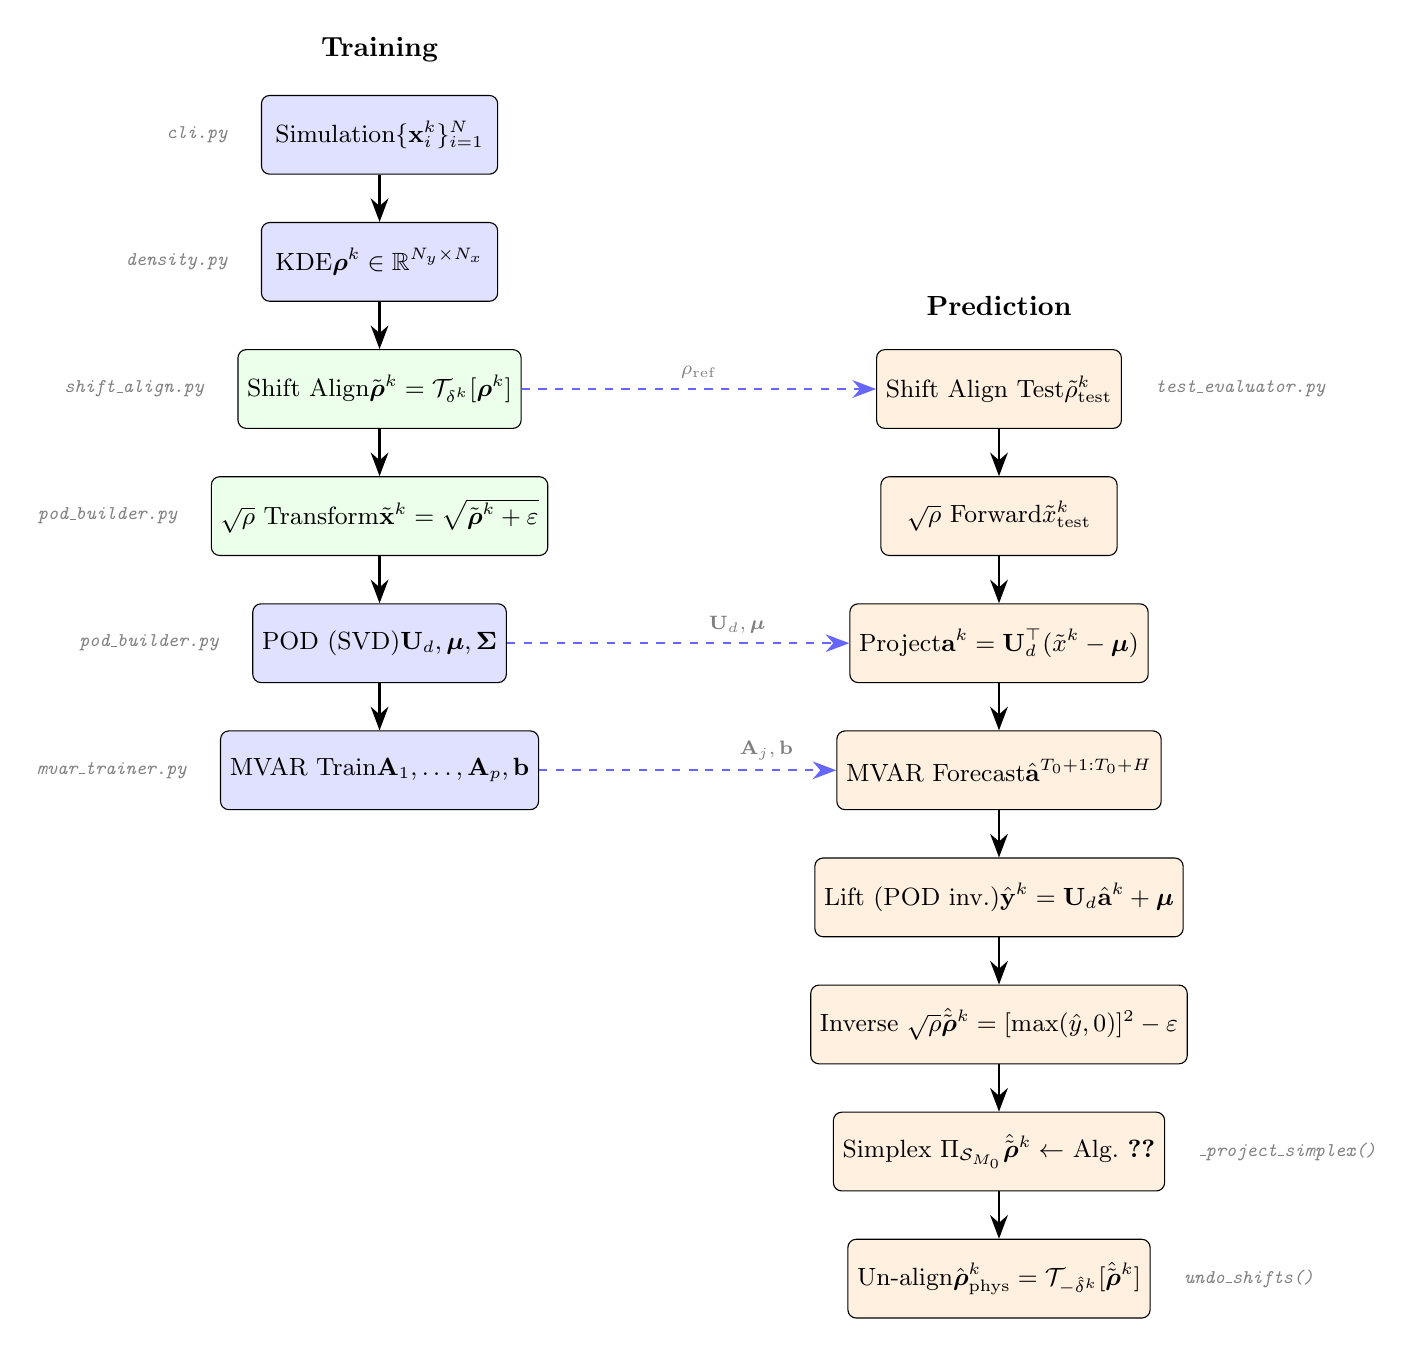
\begin{tikzpicture}[
  node distance=0.6cm and 1.5cm,
  block/.style={
    rectangle, draw, rounded corners=3pt,
    minimum height=1.0cm, minimum width=3.0cm,
    text centered, font=\small
  },
  trainblock/.style={block, fill=blue!12},
  testblock/.style={block, fill=orange!12},
  bothblock/.style={block, fill=green!8},
  arrow/.style={-{Stealth[length=3mm]}, thick},
  note/.style={font=\scriptsize\itshape, text=gray},
]

% ---- Training column (left) ----
\node[trainblock] (sim)
  {Simulation\\$\{\bx_i^k\}_{i=1}^N$};
\node[trainblock, below=of sim] (kde)
  {KDE\\$\brho^k \in \R^{N_y \times N_x}$};
\node[bothblock, below=of kde] (sa)
  {Shift Align\\$\tilde{\brho}^k = \mathcal{T}_{\delta^k}[\brho^k]$};
\node[bothblock, below=of sa] (sqrt)
  {$\sqrt{\rho}$ Transform\\$\tilde{\bx}^k = \sqrt{\tilde{\brho}^k + \varepsilon}$};
\node[trainblock, below=of sqrt] (pod)
  {POD (SVD)\\$\bU_d, \bmu, \boldsymbol{\Sigma}$};
\node[trainblock, below=of pod] (mvar)
  {MVAR Train\\$\bA_1, \ldots, \bA_p, \mathbf{b}$};

% Arrows (training)
\draw[arrow] (sim) -- (kde);
\draw[arrow] (kde) -- (sa);
\draw[arrow] (sa) -- (sqrt);
\draw[arrow] (sqrt) -- (pod);
\draw[arrow] (pod) -- (mvar);

% File labels (left)
\node[note, left=0.3cm of sim] {\texttt{cli.py}};
\node[note, left=0.3cm of kde] {\texttt{density.py}};
\node[note, left=0.3cm of sa] {\texttt{shift\_align.py}};
\node[note, left=0.3cm of sqrt] {\texttt{pod\_builder.py}};
\node[note, left=0.3cm of pod] {\texttt{pod\_builder.py}};
\node[note, left=0.3cm of mvar] {\texttt{mvar\_trainer.py}};

% ---- Prediction column (right) ----
\node[testblock, right=4.5cm of sa] (sa_test)
  {Shift Align Test\\$\tilde{\rho}_{\mathrm{test}}^k$};
\node[testblock, below=of sa_test] (sqrt_test)
  {$\sqrt{\rho}$ Forward\\$\tilde{x}_{\mathrm{test}}^k$};
\node[testblock, below=of sqrt_test] (proj)
  {Project\\$\ba^k = \bU_d^\top(\tilde{x}^k - \bmu)$};
\node[testblock, below=of proj] (forecast)
  {MVAR Forecast\\$\hat{\ba}^{T_0+1:T_0+H}$};
\node[testblock, below=of forecast] (lift)
  {Lift (POD inv.)\\$\hat{\by}^k = \bU_d \hat{\ba}^k + \bmu$};
\node[testblock, below=of lift] (inv_sqrt)
  {Inverse $\sqrt{\rho}$\\$\hat{\tilde{\brho}}^k = [\max(\hat{y},0)]^2 - \varepsilon$};
\node[testblock, below=of inv_sqrt] (simplex)
  {Simplex $\Pi_{\mathcal{S}_{M_0}}$\\$\hat{\tilde{\brho}}^k \gets$ Alg.~\ref{alg:simplex}};
\node[testblock, below=of simplex] (unalign)
  {Un-align\\$\hat{\brho}_{\mathrm{phys}}^k = \mathcal{T}_{-\hat\delta^k}[\hat{\tilde{\brho}}^k]$};

% Arrows (prediction)
\draw[arrow] (sa_test) -- (sqrt_test);
\draw[arrow] (sqrt_test) -- (proj);
\draw[arrow] (proj) -- (forecast);
\draw[arrow] (forecast) -- (lift);
\draw[arrow] (lift) -- (inv_sqrt);
\draw[arrow] (inv_sqrt) -- (simplex);
\draw[arrow] (simplex) -- (unalign);

% Cross arrows (training artifacts used at test time)
\draw[arrow, dashed, blue!60]
  (sa.east) -- node[above, note]{$\rho_{\mathrm{ref}}$} (sa_test.west);
\draw[arrow, dashed, blue!60]
  (pod.east) -- ++(1.5,0) |- node[near end, above, note]{$\bU_d, \bmu$} (proj.west);
\draw[arrow, dashed, blue!60]
  (mvar.east) -- ++(2.0,0) |- node[near end, above, note]{$\bA_j, \mathbf{b}$} (forecast.west);

% File labels (right)
\node[note, right=0.3cm of sa_test] {\texttt{test\_evaluator.py}};
\node[note, right=0.3cm of simplex] {\texttt{\_project\_simplex()}};
\node[note, right=0.3cm of unalign] {\texttt{undo\_shifts()}};

% Column headers
\node[above=0.3cm of sim, font=\bfseries] {Training};
\node[above=0.3cm of sa_test, font=\bfseries] {Prediction};

\end{tikzpicture}
\caption{Complete CrowdROM pipeline.
  \textcolor{blue!70}{Blue} = training only,
  \textcolor{orange!70}{orange} = test time only,
  \textcolor{green!50!black}{green} = shared operations.
  Dashed arrows show training artifacts consumed at test time.}
\label{fig:pipeline}
\end{figure}


% ============================================================================
\section{Configuration Summary}
% ============================================================================

All pipeline options are set in the YAML config under the \texttt{rom:} block:

\begin{table}[h]
\centering
\small
\begin{tabular}{@{}lll@{}}
\toprule
\textbf{Config Key} & \textbf{Values} & \textbf{Effect} \\
\midrule
\texttt{shift\_align}           & \texttt{true}/\texttt{false}        & Enable sPOD alignment \\
\texttt{shift\_align\_ref}      & \texttt{"mean"}, \texttt{"first"}, \texttt{"median"} & Reference field computation \\
\texttt{density\_transform}     & \texttt{"raw"}, \texttt{"sqrt"}, \texttt{"log"}       & Pre-POD transform \\
\texttt{density\_transform\_eps}& float ($10^{-10}$)                  & Regularisation $\varepsilon$ \\
\texttt{fixed\_modes}           & int or \texttt{null}                & Fixed POD rank $d$ \\
\texttt{pod\_energy}            & float ($0.99$)                      & Energy threshold if no fixed rank \\
\texttt{mass\_postprocess}      & \texttt{"none"}, \texttt{"simplex"}, \texttt{"scale"} & Post-inverse mass correction \\
\texttt{models.mvar.lag}        & int ($5$)                           & VAR order $p$ \\
\texttt{models.mvar.ridge\_alpha} & float ($10^{-4}$)                 & Ridge regularisation $\alpha$ \\
\bottomrule
\end{tabular}
\caption{Pipeline configuration keys (\texttt{rom:} section of YAML).}
\label{tab:config}
\end{table}


% ============================================================================
\section*{References}
% ============================================================================

\begingroup
\renewcommand{\section}[2]{}%
\begin{thebibliography}{99}

\bibitem[Anscombe(1948)]{Anscombe1948}
Anscombe, F.~J. (1948).
\newblock The transformation of Poisson, binomial and negative-binomial data.
\newblock \emph{Biometrika}, 35(3/4):246--254.

\bibitem[Black et~al.(2020)]{BlackVellaReiss2020}
Black, F., Schulze, P., and Reiss, J. (2020).
\newblock Projection-based model reduction with dynamically transformed modes.
\newblock \emph{ESAIM: Mathematical Modelling and Numerical Analysis},
  54(6):2011--2043.

\bibitem[D'Orsogna et~al.(2006)]{DorsognaEtAl2006}
D'Orsogna, M.~R., Chuang, Y.-L., Bertozzi, A.~L., and Chayes, L.~S. (2006).
\newblock Self-propelled particles with soft-core interactions: patterns,
  stability, and collapse.
\newblock \emph{Physical Review Letters}, 96(10):104302.

\bibitem[Duchi et~al.(2008)]{DuchiEtAl2008}
Duchi, J., Shalev-Shwartz, S., Singer, Y., and Chandra, T. (2008).
\newblock Efficient projections onto the $\ell_1$-ball for learning in high
  dimensions.
\newblock In \emph{Proceedings of the 25th International Conference on Machine
  Learning (ICML)}, pages 272--279.

\bibitem[Hastie et~al.(2009)]{HastieEtAl2009}
Hastie, T., Tibshirani, R., and Friedman, J. (2009).
\newblock \emph{The Elements of Statistical Learning}.
\newblock Springer, 2nd edition.

\bibitem[Le~Cam(1986)]{LeCam1986}
Le~Cam, L. (1986).
\newblock \emph{Asymptotic Methods in Statistical Decision Theory}.
\newblock Springer-Verlag, New York.

\bibitem[L{\"u}tkepohl(2005)]{Lutkepohl2005}
L{\"u}tkepohl, H. (2005).
\newblock \emph{New Introduction to Multiple Time Series Analysis}.
\newblock Springer-Verlag, Berlin.

\bibitem[Reiss et~al.(2018)]{ReissEtAl2018}
Reiss, J., Schulze, P., Sesterhenn, J., and Mehrmann, V. (2018).
\newblock The shifted proper orthogonal decomposition: A mode decomposition for
  multiple transport phenomena.
\newblock \emph{SIAM Journal on Scientific Computing}, 40(3):A1322--A1344.

\bibitem[Silverman(1986)]{SilvermanKDE1986}
Silverman, B.~W. (1986).
\newblock \emph{Density Estimation for Statistics and Data Analysis}.
\newblock Chapman \& Hall, London.

\bibitem[Tsybakov(2009)]{Tsybakov2009}
Tsybakov, A.~B. (2009).
\newblock \emph{Introduction to Nonparametric Estimation}.
\newblock Springer, New York.

\bibitem[Vicsek et~al.(1995)]{Vicsek1995}
Vicsek, T., Czir{\'o}k, A., Ben-Jacob, E., Cohen, I., and Shochet, O. (1995).
\newblock Novel type of phase transition in a system of self-driven particles.
\newblock \emph{Physical Review Letters}, 75(6):1226--1229.

\end{thebibliography}
\endgroup

\end{document}
